\section{Failure-mode taxonomy}
\label{sec:failure-modes}

The weighted-law derivation is not a universal raw AGOP theorem. It separates
three logically distinct bridges:
\[
H^2\approx \kappa_{\mathrm{eff}}\widetilde G,
\qquad
\widetilde G\approx \beta_{\mathrm{fit}}G,
\qquad
\beta_{\mathrm{fit}}\not\approx 0.
\]
The first bridge is the stationarity-derived weighted law. The second bridge is
the beta bridge from residual-weighted AGOP to raw AGOP. The third is a
conditioning requirement for de-weighting.

\subsection{Beta failure}

Recall the hidden-gradient leverage identity
\[
\beta_{\mathrm{fit}}
=
\frac1n\sum_i\ell_i r_i^2,
\qquad
\frac1n\sum_i\ell_i=1.
\]
Thus
\[
\beta_{\mathrm{fit}}-\bar r^2
=
\operatorname{Cov}_n(\ell,r^2),
\qquad
\bar r^2:=\frac1n\sum_i r_i^2.
\]
When empirical variances are nonzero,
\[
\frac{\beta_{\mathrm{fit}}}{\bar r^2}-1
=
\operatorname{Corr}_n(\ell,r^2)
\operatorname{CV}_n(\ell)
\operatorname{CV}_n(r^2).
\]
Therefore beta tracking fails when residual energy concentrates on
leverage-extreme samples. A rare hard cluster gives positive covariance and
overestimates mean residual energy. A high-residual low-leverage sample gives
negative covariance and underestimates it.

\subsection{Pair failure}

Let \(A=QR=U\Sigma V^\top\), and define
\[
H_X:=V^\top X^\top XV,
\qquad
F_X:=H_X-d_{\mathrm{eff}}I,
\qquad
G_{\mathrm{stat}}:=\Sigma^2V^\top X^\top.
\]
At exact \(B\)-stationarity,
\[
B^\top(S-d_{\mathrm{eff}}T)B
=
\frac1{\lambda^2n^2}
G_{\mathrm{stat}}^\top F_XG_{\mathrm{stat}}.
\]
Thus the global pair diagnostic
\[
\mathcal A_{\mathrm{pair}}=\|F_X\|_{\mathrm{op}}
\]
can be misleading in both directions. A large global defect is harmless if it is
low-gain. But a defect that is large on high-gain directions gives a genuine
failure of the weighted law.

\subsection{Raw-law conditioning failure}

Suppose
\[
\|H^2-\kappa_{\mathrm{eff}}\widetilde G\|_{\mathrm{op}}\le E_w,
\qquad
\|\widetilde G-\beta G\|_{\mathrm{op}}\le E_\beta.
\]
Then
\[
\|H^2-\kappa_{\mathrm{eff}}\beta G\|_{\mathrm{op}}
\le
E_w+\kappa_{\mathrm{eff}}E_\beta.
\]
Solving for \(G\) divides by \(|\beta|\). Hence the raw AGOP law becomes
ill-conditioned near interpolation, even if the weighted law is stable.

\subsection{Regimes}

\begin{center}
\begin{tabular}{llll}
\hline
Regime & Beta bridge & Pair closure & Raw law \\
\hline
Fully benign & holds & high-gain closure holds & holds if beta is not tiny \\
Late weighted-only & structurally holds & holds & ill-conditioned \\
Beta failure & fails high or low & may hold & biased or fails \\
Pair failure & may hold & fails on high-gain directions & fails \\
Conservative pair diagnostic & may hold & pushed error small & depends on beta \\
\hline
\end{tabular}
\end{center}

The deterministic toy figures in \autoref{fig:failure-mode-toys} illustrate
these mechanisms. They should be read as algebraic checks, not as trained-network
evidence.

\begin{figure}[h]
\centering
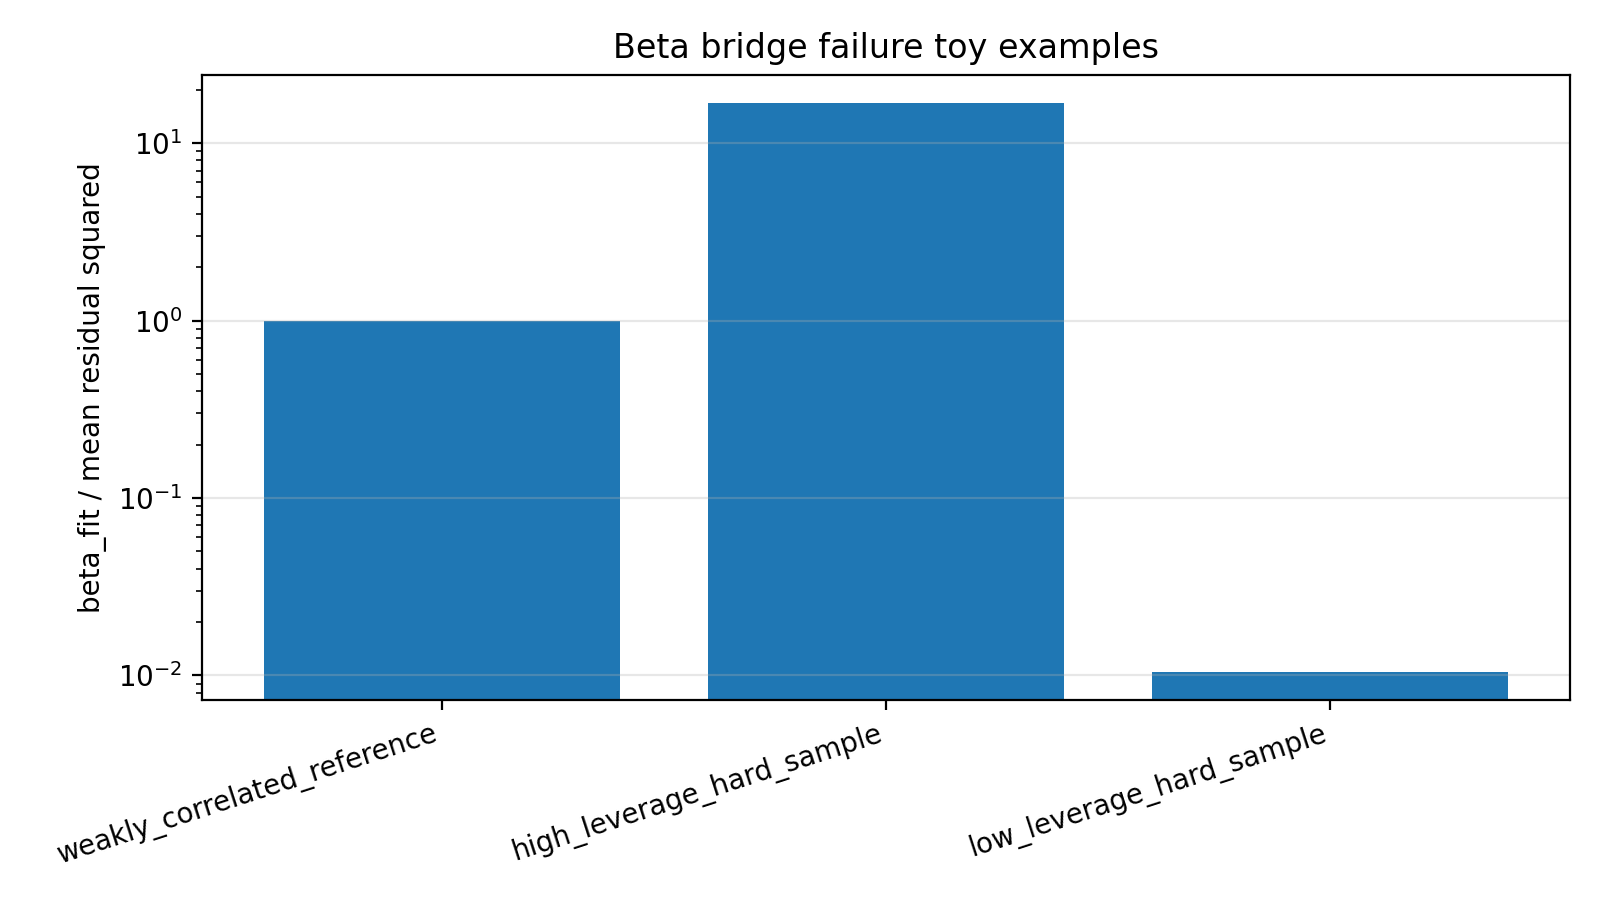
\includegraphics[width=.32\linewidth]{figures/failure_modes/beta_failure_toy.png}
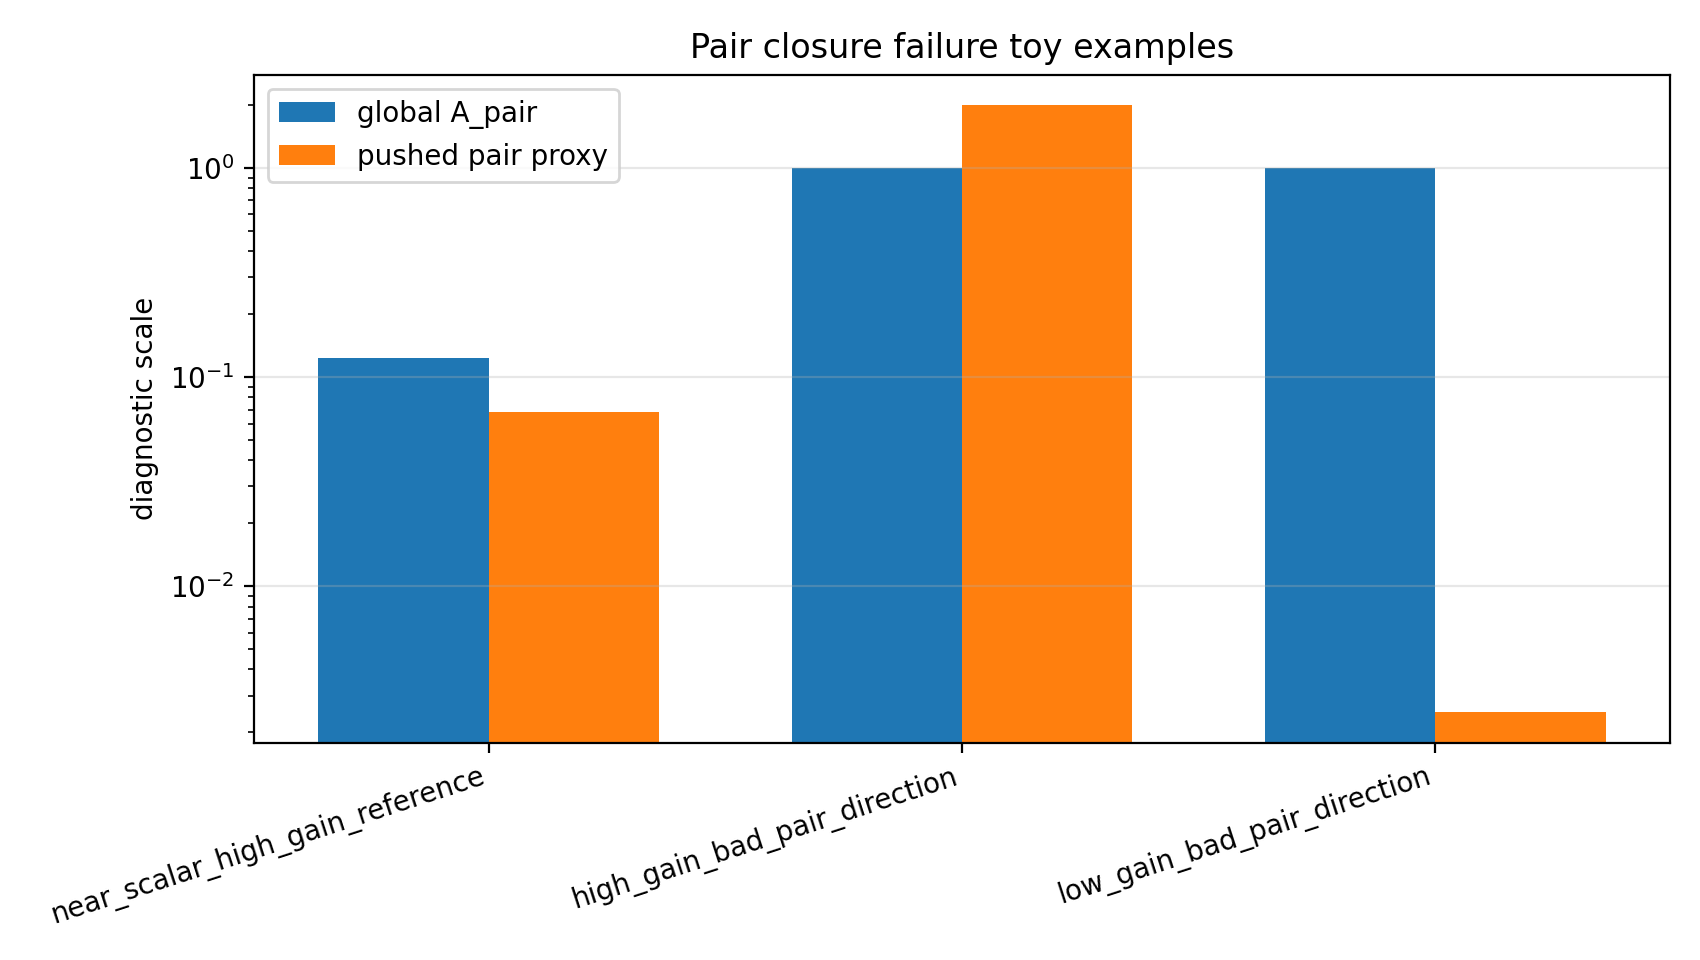
\includegraphics[width=.32\linewidth]{figures/failure_modes/pair_failure_toy.png}
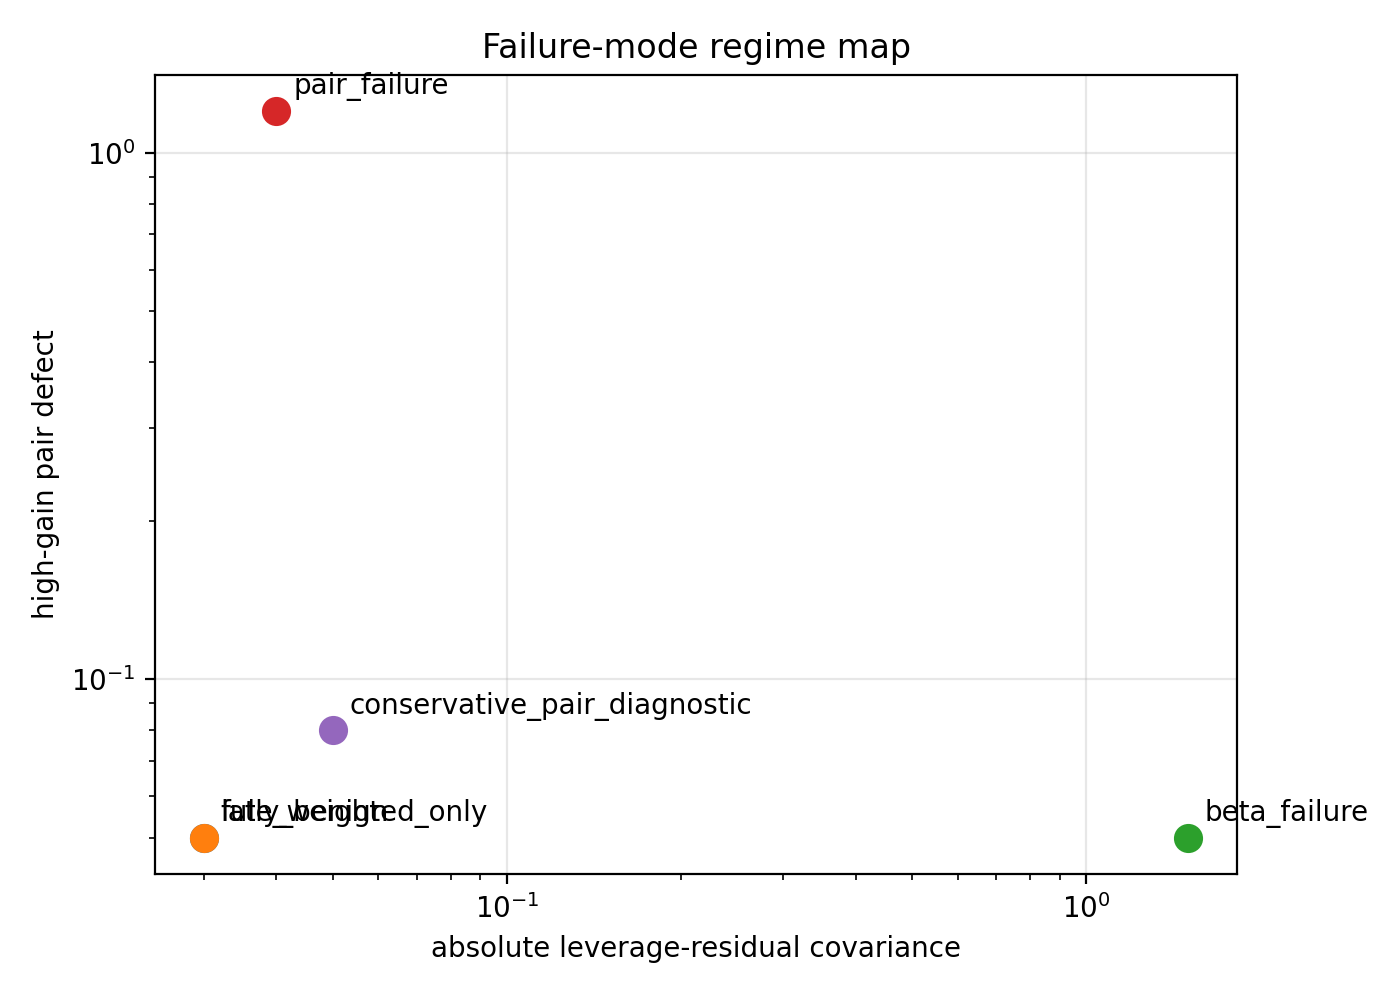
\includegraphics[width=.32\linewidth]{figures/failure_modes/regime_map.png}
\caption{Failure-mode toy diagnostics. Left: beta tracking can overestimate or
underestimate mean residual energy when leverage and residual energy couple.
Middle: global pair defect is not enough, since the pushed pair proxy depends on
stationarity gain. Right: a conceptual map of regimes by beta covariance and
high-gain pair defect.}
\label{fig:failure-mode-toys}
\end{figure}

\subsection{Status}

The taxonomy proves that universal raw AGOP claims are impossible without bridge
assumptions. It does not prove that trained networks enter a specific regime.
The trained synthetic failure families are empirical probes for whether rare
regions, mixture subspaces, and gated tasks realize the algebraic mechanisms.
